%%%%%%%%%%%%%%%%%%%%%%%% ExtendedAbstract.tex %%%%%%%%%%%%%%%%%%%%%%%%
%                                                                    %
%  Template for the 10-page extended abstract to be submitted for    %
%  the MSc degree conferral at Instituto Superior Tecnico.           %
%                                                                    %
%  Author:                                                           %
%                                                                    %
%       Andre C. Marta                                               %
%       Area Cientifica de Mecanica Aplicada e Aeroespacial          %
%       Departamento de Engenharia Mecanica                          %
%       Instituto Superior Tecnico                                   %
%       Av. Rovisco Pais                                             %
%       1049-001 Lisboa                                              %
%       Portugal                                                     %
%       Tel: +351 21 841 9466                                        %
%                        3466 (extension)                            %
%       Email: andre.marta@ist.utl.pt                                %
%                                                                    %
%  Created:       Dec  2, 2011                                       %
%  Last Modified: Dec 27, 2011                                       %
%%%%%%%%%%%%%%%%%%%%%%%%%%%%%%%%%%%%%%%%%%%%%%%%%%%%%%%%%%%%%%%%%%%%%%
% This document uses the LaTeX class file "article.cls"              %
%%%%%%%%%%%%%%%%%%%%%%%%%%%%%%%%%%%%%%%%%%%%%%%%%%%%%%%%%%%%%%%%%%%%%%
\documentclass[10pt,a4paper,twocolumn]{article}

%%%%%%%%%%%%%%%%%%%%%%%%%%%%%%%%%%%%%%%%%%%%%%%%%%%%%%%%%%%%%%%%%%%%%%
% Document preamble
%%%%%%%%%%%%%%%%%%%%%%%%%%%%%%%%%%%%%%%%%%%%%%%%%%%%%%%%%%%%%%%%%%%%%%

%% Builds upon the graphics  package, providing a key-value interface
%% for optional arguments to the \includegraphics command that go far
%% beyone what the graphics package offers.
%% http://www.ctan.org/tex-archive/help/Catalogue/entries/graphicx.html
%% if you use PostScript figures in your article
%% use the graphics package for simple commands
%% \usepackage{graphics}
%% or use the graphicx package for more complicated commands
%% \usepackage{graphicx}
%% or use the epsfig package if you prefer to use the old commands
%% \usepackage{epsfig}
\usepackage{graphicx} % Enhanced LaTeX Graphics

% Multiple figures
\usepackage{subfigure} % subcaptions for subfigures
\usepackage{subfigmat} % matrices of similar subfigures

% Declaring new column types
% 'dcolumn' package defines D to be a column specifier with
% three arguments: D{<sep.tex>}{<sep.dvi>}{<decimal places>}
%                  D{<sep.tex>}{<sep.dvi>}{<left digit places>.<right digit places>}
\usepackage{dcolumn}           % decimal-aligned tabular math columns
% d takes a single argument specifying the number of decimal places, e.g., d{2}
% or the number of digits to the left and right of the seperator, e.g., d{3.2}
\newcolumntype{.}   {D{.}{.}{-1}} % column alignedd on the point separator '.'
\newcolumntype{d}[1]{D{.}{.}{#1}} % column centered on the point separator '.'
\newcolumntype{e}   {D{E}{E}{-1}} % column centered on the exponent 'E'
\newcolumntype{E}[1]{D{E}{E}{#1}} % column centered on the exponent 'E'

\usepackage{titlesec}
\usepackage{booktabs}
\usepackage{multirow}
\usepackage{xcolor}
\usepackage{color}
\usepackage{colortbl}
\PassOptionsToPackage{hyphens}{url}\usepackage{hyperref}
\definecolor{forestgreen}{RGB}{34,139,34}
\definecolor{orangered}{RGB}{239,134,64}
\definecolor{lightred}{rgb}{1,0.4,0.5}
\definecolor{orange}{rgb}{1,0.45,0.13}	
\definecolor{darkblue}{rgb}{0.0,0.0,0.6}
\definecolor{lightblue}{rgb}{0.1,0.57,0.7}
\definecolor{gray}{rgb}{0.4,0.4,0.4}
\definecolor{lightgray}{rgb}{0.95, 0.95, 0.95}
\definecolor{darkgray}{rgb}{0.4, 0.4, 0.4}
\definecolor{editorGray}{rgb}{0.95, 0.95, 0.95}
\definecolor{editorOcher}{rgb}{1, 0.5, 0} % #FF7F00 -> rgb(239, 169, 0)
\definecolor{chaptergrey}{rgb}{0.6,0.6,0.6}
\definecolor{editorGreen}{rgb}{0, 0.5, 0} % #007C00 -> rgb(0, 124, 0)
\definecolor{olive}{rgb}{0.17,0.59,0.20}
\definecolor{brown}{rgb}{0.69,0.31,0.31}
\definecolor{purple}{rgb}{0.38,0.18,0.81}
\usepackage[ruled,vlined,norelsize,\languagename]{algorithm2e}

%% American Mathematical Society (AMS) plain Tex macros
%%
%% The amsmath package is the principal package in the AMS-LaTeX distribution
%% http://www.ctan.org/tex-archive/help/Catalogue/entries/amsmath.html
\usepackage{amsmath}
%%
%% The amsfonts package provides extended TeX fonts
%% http://www.ctan.org/tex-archive/help/Catalogue/entries/amsfonts.html
\usepackage{amsfonts}
%% The amssymb package provides various useful mathematical symbols
\usepackage{amssymb}
%%
%% The amsthm package provides extended theorem environments
%% http://www.ctan.org/tex-archive/help/Catalogue/entries/amsthm.html
\usepackage{amsthm}

%% Improves the interface for defining floating objects such as figures and tables.
%% The package also provides the H float modifier option of the obsolete here package.
%% http://www.ctan.org/tex-archive/help/Catalogue/entries/float.html
\usepackage{float}

%% Control sectional headers. 
%% http://www.ctan.org/tex-archive/help/Catalogue/entries/sectsty.html
\usepackage{sectsty}
%%
%% Redefine the font size of the 'section' and 'subsection' headings
\newcommand{\myFontSize}{\fontsize{10}{0}\selectfont}
\sectionfont{\myFontSize}       % 10pt, Bold face (default)
\subsectionfont{\rm\myFontSize} % 10pt, Plain face

%% Select alternative section titles.
%% http://www.ctan.org/tex-archive/help/Catalogue/entries/titlesec.html
\usepackage{titlesec}
%%
%% Left indent, before and after spacing
%% (The starred version kills the indentation of the paragraph following the title)
\titlespacing*{\section}{0pt}{10pt}{0pt}
\titlespacing*{\subsection}{0pt}{10pt}{0pt}

%% Section numbers with trailing dots. 
%% http://www.ctan.org/tex-archive/help/Catalogue/entries/secdot.html
\usepackage{secdot}
%%
%% Also put a dot after the subsection number
\sectiondot{subsection}
%% Set a space between dot and heading text
\sectionpunct{section}{. }    % By default, \sectiondot places a \quad
\sectionpunct{subsection}{. } % after the number

% These are exact settings for a A4 page with top margin of
% 25 mm, bottom margin of 30 mm, left and right margins of 25 mm,
% printable area 242 X 160 mm.

\setlength{\topmargin}{-10.4mm}
\setlength{\headheight}{0.0mm}
\setlength{\headsep}{10.0mm}
\setlength{\textwidth}{160mm}
\setlength{\textheight}{242mm}
\setlength{\oddsidemargin}{0mm}
\setlength{\evensidemargin}{0mm}
\setlength{\marginparwidth}{0mm}
\setlength{\marginparsep}{0mm}

% New command to refer to equations as Eq.(1),Eq.(2),...
\newcommand{\eqnref}[1]{Eq.(\ref{#1})}

%%%%%%%%%%%%%%%%%%%%%%%%%%%%%%%%%%%%%%%%%%%%%%%%%%%%%%%%%%%%%%%%%%%%%%%%%%%%%%%%%%%%%%%%
% Title, authors and addresses

\title{Air Quality Monitoring and Interpolation System for IoT Applications}
\date{December 2019}
\author{Bernardo Nuno Bernardo Amaral \\ bernardo.amaral@ist.utl.pt \\ \\ Instituto Superior T\'{e}cnico, Lisboa, Portugal}

%%%%%%%%%%%%%%%%%%%%%%%%%%%%%%%%%%%%%%%%%%%%%%%%%%%%%%%%%%%%%%%%%%%%%%%%%%%%%%%%%%%%%%%%
\begin{document}

% Begin one column section for title and abstract
%
% http://www.faqs.org/faqs/de-tex-faq/part5/
%\twocolumn[
%\begin{@twocolumnfalse}
\maketitle

%%%%%%%%%%%%%%%%%%%%%%%%%%%%%%%%%%%%%%%%%%%%%%%%%%%%%%%%%%%%%%%%%%%%%%
% ABSTRACT & KEYWORDS
%%%%%%%%%%%%%%%%%%%%%%%%%%%%%%%%%%%%%%%%%%%%%%%%%%%%%%%%%%%%%%%%%%%%%%
%%%%%%%%%%%%%%%%%%%%%%%%%%%%%%%%%%%%%%%%%%%%%%%%%%%%%%%%%%%%%%%%%%%%%%
%     File: ExtendedAbstract_abstr.tex                               %
%     Tex Master: ExtendedAbstract.tex                               %
%                                                                    %
%     Author: Andre Calado Marta                                     %
%     Last modified : 2 Dez 2011                                     %
%%%%%%%%%%%%%%%%%%%%%%%%%%%%%%%%%%%%%%%%%%%%%%%%%%%%%%%%%%%%%%%%%%%%%%
% The abstract of should have less than 500 words.
% The keywords should be typed here (three to five keywords).
%%%%%%%%%%%%%%%%%%%%%%%%%%%%%%%%%%%%%%%%%%%%%%%%%%%%%%%%%%%%%%%%%%%%%%

%%
%% Abstract
%%
\begin{abstract}
Air pollution is a global problem due to its consequences on population health. World Health Organization estimates that every year 7 million deaths are caused by air pollution related to small inhalable particles. This work intends to provide useful research in the scope of air pollution monitoring and spatial prediction, through the development of a pioneer Narrow-band Internet of Things (NB-IoT) based system for the measurement of particulate matter with a diameter smaller than 10 micrometers, using the low-cost PMS5003 sensor. This system integration in official monitoring clusters was tested, through the comparison with the Portuguese Environment Agency reference sensors in Lisbon, aiming to improve the spatial density of the current network. Furthermore, to enhance the resolution of available data, several algorithms, such as Ordinary Kriging, Inverse Distance Weighting, Linear Interpolation, Nearest Neighbors and Fuzzy Boolean Nets were tested for spatial interpolation through cross-validation, with data from 2013 to 2017. Finally, a web platform for the visualization of live interpolated PM10 concentration was produced. NB-IoT presented low coverage in the city, and comparisons between sensor measurements showed several inconsistencies in the low-cost sensor. Ordinary Kriging and Inverse Distance Weighting, with a zero power function, presented the best performance, indicating a low distance correlation between the reference stations. The developed application allowed a successful representation of high resolution interpolated data. Currently, the NB-IoT technology is not well established in Portugal and further research is needed to improve the integration of low-cost solutions in air quality monitoring networks.\\
%%
%% Keywords (max 5)
%%
\noindent{{\bf Keywords:}} Air Quality, Particulate Matter, Spatial Interpolation Models, Fuzzy Boolean Nets, LPWAN, NB-IoT \\

\end{abstract}



% End one column section (begin default two columns)
%\end{@twocolumnfalse}
%]
%%%%%%%%%%%%%%%%%%%%%%%%%%%%%%%%%%%%%%%%%%%%%%%%%%%%%%%%%%%%%%%%%%%%%%
% INTRODUCTION
%%%%%%%%%%%%%%%%%%%%%%%%%%%%%%%%%%%%%%%%%%%%%%%%%%%%%%%%%%%%%%%%%%%%%%
\section{Introduction}
\label{sec:intro}

In the present days, air pollution is a major environmental problem. In 2016, it was responsible for approximately 4.2 million deaths and is currently estimated to be accountable for 25\% of adult deaths from strokes, 43\% from chronic obstructive pulmonary disease and 29\% from lung cancer \cite{WHO2018}. It is also responsible for stunting plant growth, lowering agricultural productivity and for reducing city growth and attractiveness to citizens, slowing their evolution and development \cite{GSMA2018}.

At the time of this work, systems for the measurement of air pollution are placed in urban environments as an investment made in the last two decades addressing the emerging knowledge on air pollution health hazards. These systems are constituted by container-style monitoring stations, which occupy large spaces, have high power consumption and high maintenance and production costs. In the greater Lisbon area, there are only fourteen air pollution monitoring stations. From these, only thirteen measure particulate matter with a diameter smaller than 10 micrometers (PM10) and only four measure particulate matter with a diameter smaller than 2.5 micrometers (PM2.5). The monitoring station’s network completed 72 stations in 2005, in the overall area of Portugal \cite{APA2008}.

The goal of this work is to develop a system to improve the resolution of the visualization of PM10 concentration levels throughout the greater area of Lisbon, with the use of the latest Internet of Things (IoT) technologies available, machine learning and a web application. First, a low-cost portable IoT particulate matter (PM) monitoring system will be assembled. Second, with the help of the Lisbon air quality measures and data from Portuguese Online Database on Air Quality (QualAr) several Spatial Interpolation Models (SIM) will be assessed and compared with Fuzzy Boolean Nets (FBN) in what regards spatial interpolation performance. Finally, a web application that presents live, fine resolution, interpolated data of PM10 concentration in the city of Lisbon will be developed.


%%%%%%%%%%%%%%%%%%%%%%%%%%%%%%%%%%%%%%%%%%%%%%%%%%%%%%%%%%%%%%%%%%%%%%
% BACKGROUND
%%%%%%%%%%%%%%%%%%%%%%%%%%%%%%%%%%%%%%%%%%%%%%%%%%%%%%%%%%%%%%%%%%%%%%
% A Theory section should extend, not repeat, the background to the
% article already dealt with in the Introduction and lay the
% foundation for further work.

\section{Background}
\label{sec: backg}
\subsection{PM Monitoring Sensors}

Despite their price, low-cost optical PM monitors have shown to be able to characterize PM concentrations with high resolution. Recent studies show that these perform with adequate precision for indoor air monitoring, although with some calibration requirements \cite{Manikonda2016}, having also demonstrated overall good correlations with reference monitors \cite{Sayahi2018}. Additionally, it has been concluded that comprehensive understanding of the sensor characteristics is necessary and that one big disadvantage is the non-guaranteed accuracy and the lack of established scientific literature regarding these equipments \cite{Kuula2019}.

Zheng et al., in 2018, tested how environment circumstances affect these sensors performance. Results showed that relative humidity (RH) has a major influence in the sensor readings, while the temperature effects were negligible \cite{Zheng2018}.

\subsection{Interpolation Algorithms for Spatial Analysis}

Spatial interpolation consists of estimating the value of measures of certain properties, at unsampled locations, within the area covered by existing observations of the same properties. Some of the most popular spatial interpolation algorithms (SIM) are inverse distance weighting (IDW), kriging, shape functions, spline, and trend surface \cite{Li2008}.

In 2014, Li and Heap made a review of the 25 most commonly applied SIMs \cite{Li2014}. As result, an easy to use decision tree was created for use case dependent method selection. The most suitable interpolation algorithms in circumstances such as the ones in this work are IDW and ordinary kriging (OK), depending on data selection and availability, according to the decision tree.

\subsubsection{Fuzzy Boolean Nets}

FBNs are Boolean networks developed and studied by researchers at Instituto Superior Técnico \cite{Tome}. In these networks, each neuron has a binary value and is constituted by a binary table with a user-defined length. 

The networks are constituted by several neuronal areas. Each area has the same number of neurons and can only be one of two types, antecedent or consequent. 

Connections between neurons are weightless, temporary and only appear between neurons located in different areas of different types. In Figure \ref{fig:fbn-drawing}, a simple example of an FBN is presented, with two antecedent areas and one consequent area, each with four neurons.

\begin{figure}[ht]
\centering
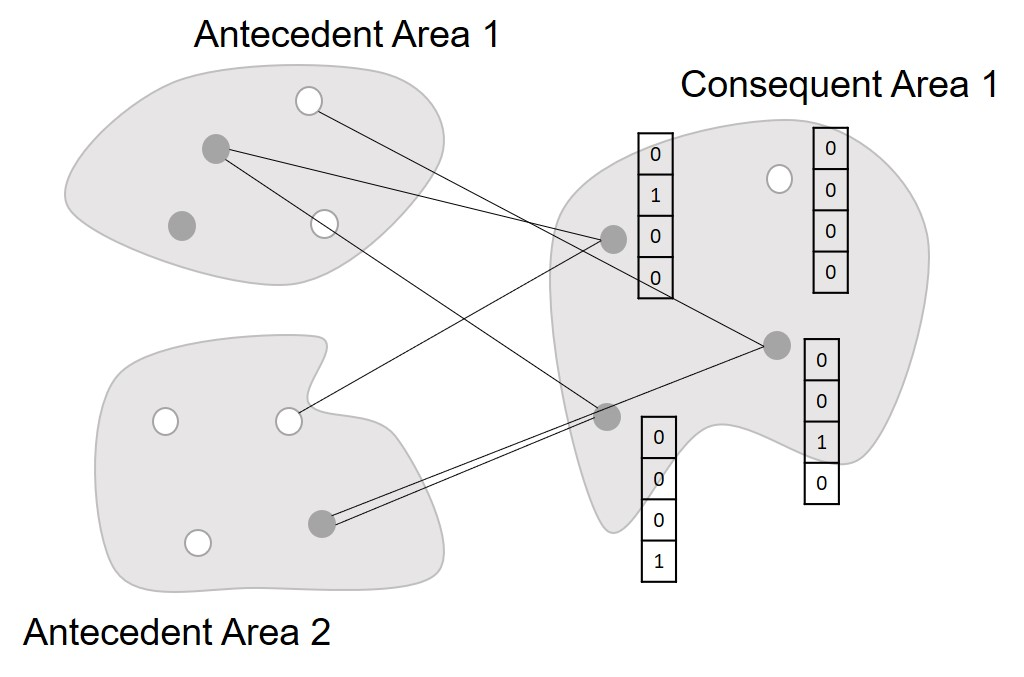
\includegraphics[width=0.45\textwidth]{./Images/fbn-drawing-2.jpg}
\caption{Example of the constituents of an FBN.}
\label{fig:fbn-drawing}
\end{figure}

The values of training and testing variables are attributed as an activation ratio to each area.

The inference process results of learning and testing epochs where consequent neurons sample an user-defined number of antecedent neurons, and according to these samples, fill their binary tables, in the training process, or retrieve a value from it, in the testing process. The final activation ratio of consequent areas represent the inference results. 

In previous studies, FBNs have shown to have positive interpolation capabilities when tested with sparse datasets \cite{Tome2014}.

\subsubsection{IDW}

IDW is a deterministic SIM based only on the assumption that the degree of influence of nearby sample points should be greater than the effect of farthest points. The only parameter which is user-defined in the IDW implementation is the power function, which defines the relevance of the distance in the calculation of the weights of each observed value \cite{Mesquita2009}.

The IDW interpolation can be defined by the equation \eqref{idw}, where \eqref{idw-weight} represents the weights associated to each observation.

\begin{equation} 
\label{idw}
\scalebox{1.2}{ $ f(x, y) = \dfrac{\sum_{i=1}^{n} w(d_i)z_i}{\sum_{i=1}^{n} w(d_i)}, i = 1, 2, ..., n$}
\end{equation}

\begin{equation} 
\label{idw-weight}
\scalebox{1.2}{ $w(d_i)= \dfrac{1}{{d_i}^{p}}$}
\end{equation}

Where $z_i$ is the observed value, $d_i$ is the distance between the estimation and the observation points, $w(d_i)$ represents the weight associated to observation \textit{i} and \textit{p} is the power function.

\subsubsection{Ordinary Kriging}

Kriging geostatistical schemes are stochastic, local, gradual and exact interpolators. In kriging, weights are based not only in the distance between points but also in the overall spatial arrangement of the observation points \cite{Mesquita2009}.

Before its application, an exploratory statistical analysis of data must be made, as well as the modelling of a variogram to represent how semivariance varies with distance.

In Figure \ref{fig:variogram}, an example of a variogram is presented. The nugget represents the semivariance value when the distance tends to zero. The sill is the point where semivariance stabilizes, and range is the interval in which, as distance increases, higher is the semivariance. Kriging interpolation weights are chosen using the modeled variogram so that estimates are unbiased and the estimation variance is minimized.

\begin{figure}[ht]
\centering
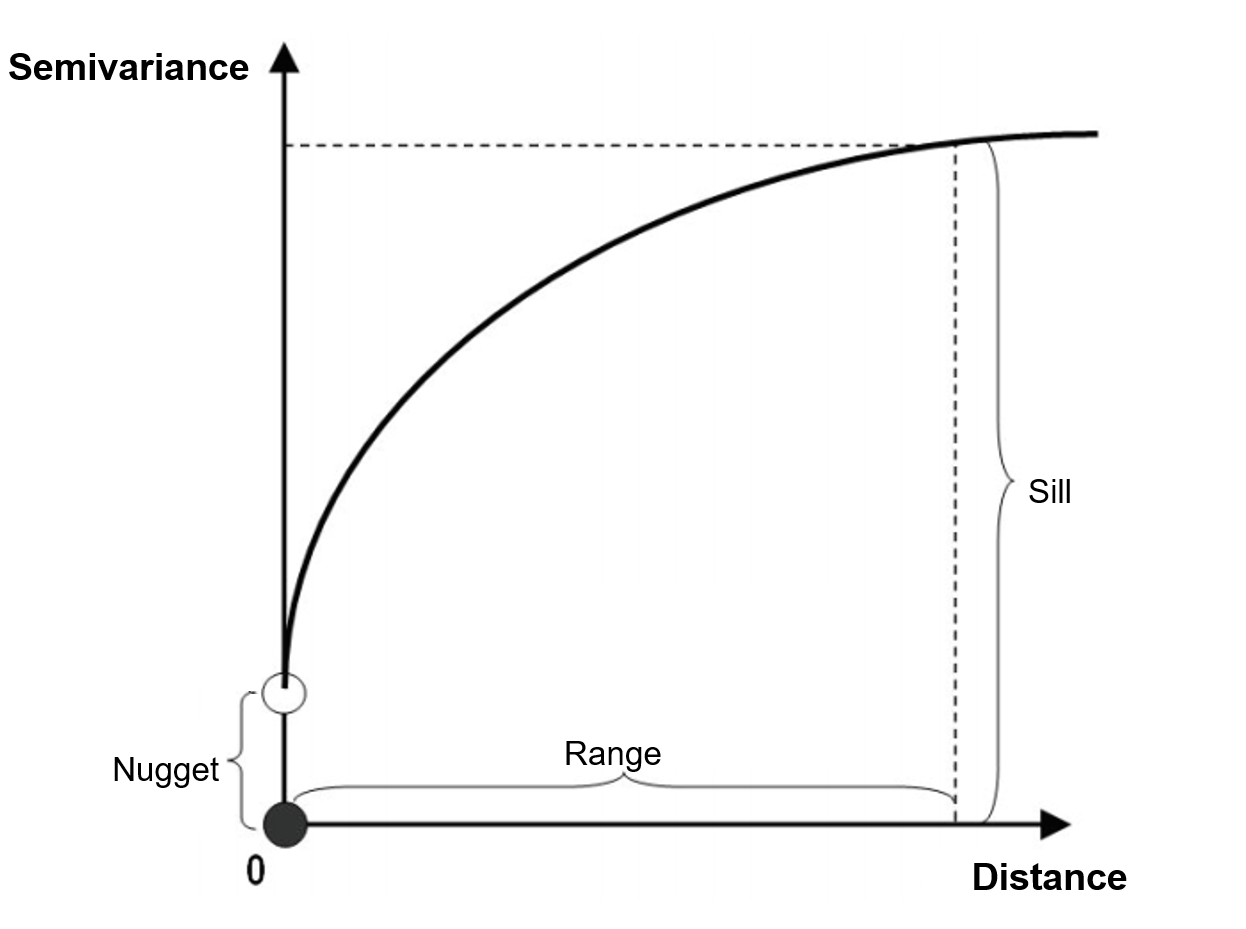
\includegraphics[width=0.49\textwidth]{./Images/variogram.png}
\caption{Example of a kriging variogram.}
\label{fig:variogram}
\end{figure}

\subsection{NB-IoT}

NB-IoT is a Low Power Wide Area Network (LPWAN) technology created in 2015 to face the growing massive IoT connectivity challenge. It operates on 180 kHz bandwidth for both downlink and uplink. The downlink remains with the same structure as Long Term Evolution (LTE) (orthogonal frequency-division multiple access (OFDMA) with 15 kHz sub-carrier spacing), and the uplink is single-carrier frequency-division multiple access (SC-FDMA) with sub-carrier spacing at 3.75 kHz (15 kHz for in-band to avoid interference from other LTE traffic) \cite{Ratasuk2016}.

Studies have compared NB-IoT to other LPWANs, such as SigFox, Long Term Evolution for Machines (LTE-M) and Long Range Wide Area Network (LORAWAN), and several advantages were observed over the latter. Some of these are that NB-IoT is more robust in terms of packet error rate \cite{Mroue2018}, it provides the best coverage, even in indoor scenarios \cite{Lauridsen2017}, and is the most suitable for IoT personal and public applications \cite{Zanella2016}.

\subsection{Air Pollution Visualization}

Currently there are two types of platforms for the visualization of live air quality data: governmental and private companies platforms.

Reviewed governmental platforms do not show fine interpolated data in their air quality live maps \cite{QualAr} \cite{U.S.EnvironmentProtectionAgency}. Instead, low resolution maps that do not show air quality variances between stations are presented. On the other hand, business oriented platforms take advantage of the publicly available air quality data provided by governments to make their live interpolated air pollution maps as a products. These represent maps with much finer resolution, but the algorithms used for the interpolation are proprietary \cite{Breezometer}.



%%%%%%%%%%%%%%%%%%%%%%%%%%%%%%%%%%%%%%%%%%%%%%%%%%%%%%%%%%%%%%%%%%%%%%
% IMPLEMENTATION
%%%%%%%%%%%%%%%%%%%%%%%%%%%%%%%%%%%%%%%%%%%%%%%%%%%%%%%%%%%%%%%%%%%%%%
\section{PM10 Monitoring, Interpolation and Visualization System}
\label{sec: imple}

The methodologies and implementation details concerning the systems developed in this work are presented and explained in this section.

\subsection{PM10 Monitoring System Assembly}

The low-cost PM10 monitoring system consists of a PM10 sensor, a microcontroller board with a NB-IoT chipset and a step-up voltage converter.
The PM10 sensor used was the PMS5003, a low-cost light-scattering optical sensor, which outputs its measures through a digital signal, processed by a microprocessor in real-time. It operates in temperatures between -10ºC and 60ºC, and relative humidity from 0 to 99\%.

The development board used was SODAQ SFF R412M, which has low power consumption and allows the use of both NB-IoT and LTE-M technologies. It contains an integrated micro-controller, the Atmel SAMD21, which allows it to be programmed through the same
tools as Arduino compatible boards.

Subscriber identity module cards provided by the mobile operators NOS and Altice Portugal were used for this board NB-IoT remote communications. These cards were previously configured by the mobile operators according to the specifications needed for its optimal use in NB-IoT devices. AT commands are used to communicate through the NB-IoT module. The commands used in the implementation of the developed system, and in the micro-controller program, along with its purpose are presented in Table \ref{table:atCommands}.

\begin{table}[ht]
\footnotesize
\centering
\caption{AT commands used with the NB-IoT micro-controller.}
\label{table:atCommands}
\begin{tabular}{l>{\raggedright\arraybackslash}p{0.33\textwidth}} % centered columns (4 columns)
\toprule
Command&Functionality\\
\midrule
AT+CFUN&Set the mobile terminal on\\
AT+CGATT&GPRS Attach\\
AT+USOCR&Create a socket\\
AT+USOST&Write to a remote address\\
AT+USOCL&Close socket\\
\bottomrule
\end{tabular}
\end{table}

The resulting system is presented in Figure \ref{fig:ieec5}. Two holes were made in the enclosure box to allow the airflow in the inlet and outlet of the sensor.

The development board was programmed, through the Arduino IDE, to collect data from the sensor, calculate 15 minute averages and send them to a server, which stores them in a database, replicating the behaviour of official monitoring networks systems. The server was developed in python, with the usage of UDP sockets, and the used database was MongoDB. 

\begin{figure}[ht]
\centering
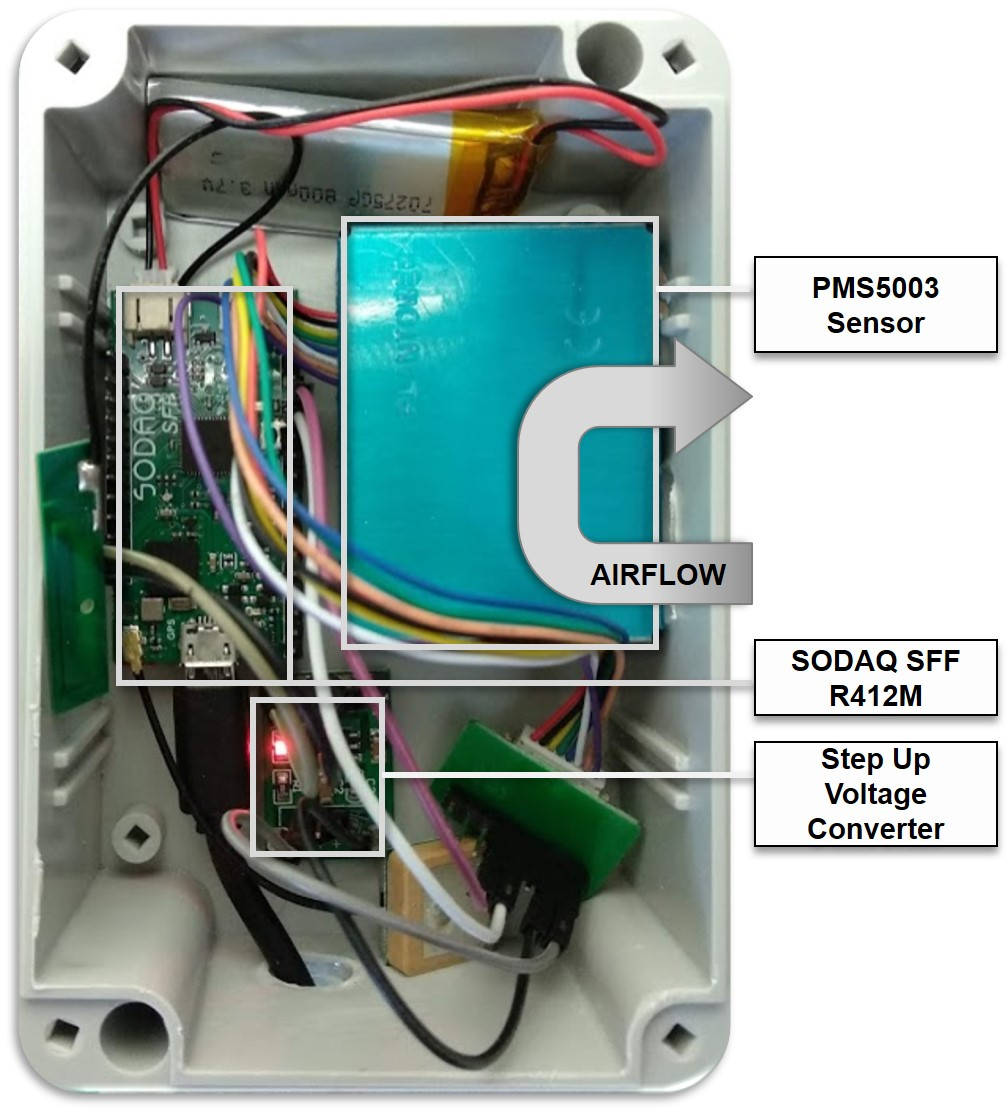
\includegraphics[width=0.49\textwidth]{./Images/circuit-final.jpg}
\caption{Developed PM monitoring system.}
\label{fig:ieec5}
\end{figure}

\subsection{Dataset Selection}

Only data from 2013 to 2017 was collected from Portuguese Online Database on Air Quality (QualAr) database, since it is the most consistent, with measures from the considered stations at high percentages of completeness.

Data was filtered to only concern monitoring stations in the greater area of Lisbon, since that is the area where these have the most spatial density in Portugal. The air quality monitoring network in the greater area of Lisbon is composed of 14 monitoring stations. Only 13 of these have operating PM10 sensors, and only 4 have operating PM2.5 sensors, with several of these lacking registered data in some years. The stations considered in this work are presented in Table \ref{table:completeness}.

\begin{table}[!htbp]
\footnotesize
\centering
\caption{Lisbon PM10 stations characterization and completeness in the dataset.}
\label{table:completeness}
\begin{tabular}{l>{\centering}p{0.06\textwidth}>{\centering}p{0.07\textwidth}>{\centering\arraybackslash}p{0.07\textwidth}}
\toprule
\multirow{2}{*}{Station}&\multirow{2}{*}{ID}&\multicolumn{2}{c}{Completeness (\%)}\\\cline{3-4}
&&Overall&Filtered\\
\midrule
Alfragide/Amadora&ALF&1.40&2.85\\
Alverca&ALV&97.47&99.96\\
Avenida da Liberdade&AVL&96.49&99.21\\
Entrecampos&ENC&76.40&99.50\\
Loures-Centro&LOC&85.88&91.46\\
Mem Martins&MEM&88.31&99.72\\
Odivelas-Ramada&ODI&82.89&98.88\\
Olivais&OLI&93.74&99.54\\
Quinta do Marquês&QMA&89.30&99.55\\
Reboleira&REB&68.88&96.88\\
Restelo&RES&29.66&40.81\\
Santa Cruz de Benfica&SCB&48.67&82.00\\
\bottomrule
\end{tabular}
\end{table}%

Further filtering was applied, data from the stations in Alverca and Alfragide was removed, due to lack of completeness in the dataset and sparse positioning, respectively. 

The objective of increasing percentages of data completeness, for every station in the dataset, was accomplished with the results of Table \ref{table:completeness}. The final dataset contained data regarding 11 657 time intervals.
%, as presented in Figure %\ref{fig:dataset-filtering}, corresponding to %the same number of total hours of PM10 %measurement of the Lisbon monitoring network.
%
%\begin{figure}[ht]
%\centering
%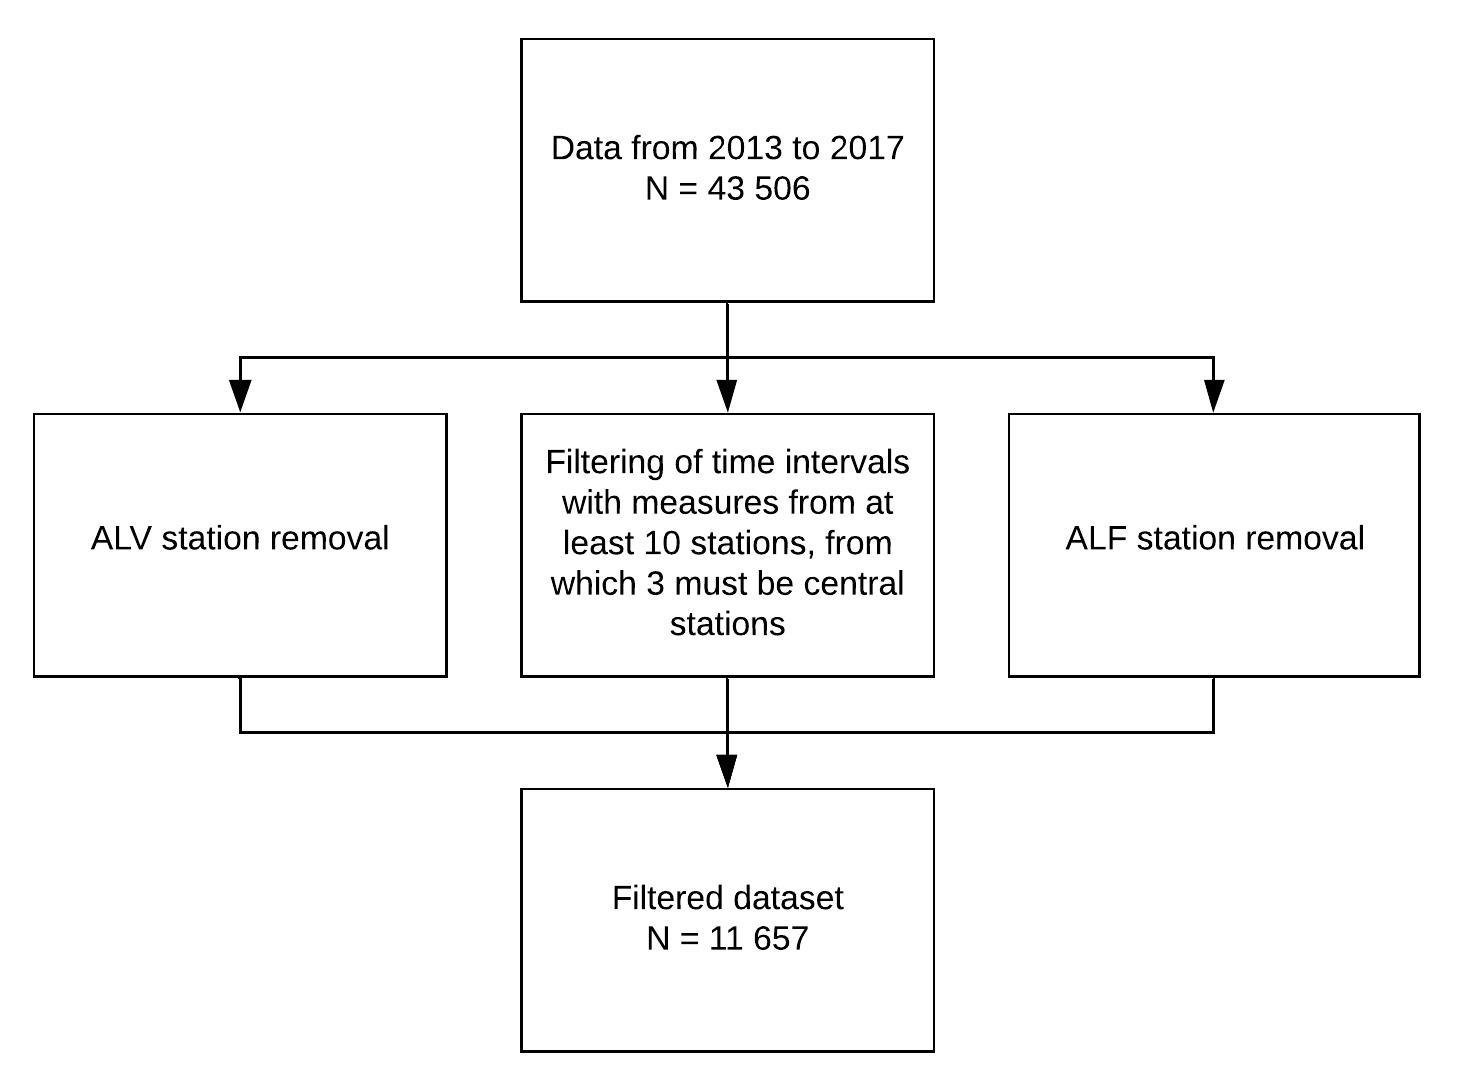
\includegraphics[width=0.49\textwidth]{./Images%/dataset-filtering.jpeg}
%\caption{Dataset exclusion process.}
%\label{fig:dataset-filtering}
%\end{figure}

The geographical location of the stations chosen for algorithm testing can be observed in Figure \ref{fig:map-filtered}, as well as, in red, the stations which are in the inside of the network outline, which will be used as infer targets.

\begin{figure}[ht]
\centering
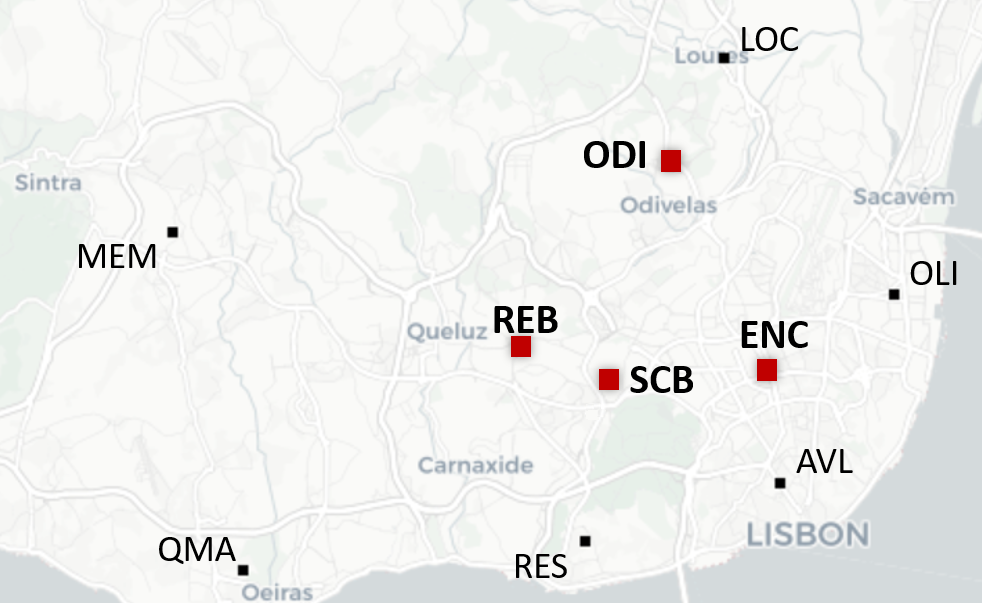
\includegraphics[width=0.46\textwidth]{./Images/map-filtered.png}
\caption{Selected stations, in the greater area of Lisbon.}
\label{fig:map-filtered}
\end{figure}

In the final filtered dataset, the Pearson coefficient was calculated between every station and every inference target station, as one can see in Table \ref{table:correlation-coef}. Possible resulting values vary from 1 to -1, where 1 represents total positive linear correlation, 0 represents no linear
correlation, and -1 total negative linear correlation.

\begin{table}[!htbp]
\centering
\footnotesize
\caption{Pearson correlation coefficients between stations.}
\label{table:correlation-coef}
\begin{tabular}[t]{l>{\centering}p{0.15\linewidth}>{\centering}p{0.15\linewidth}>{\centering}p{0.15\linewidth}>{\centering\arraybackslash}p{0.15\linewidth}}
\toprule
&ENC&ODI&REB&SCB\\
\midrule
%ALF&1&0.53&0.47&0.42&0.54\\
%ALV&0.76&0.78&0.79&0.69\\
AVL&0.83&0.77&0.78&0.76\\
ENC&1&0.84&0.82&\textbf{0.81}\\
LOC&0.77&0.79&0.79&0.69\\
MEM&0.77&0.78&0.8&0.66\\
ODI&\textbf{0.84}&1&\textbf{0.86}&0.78\\
OLI&0.83&0.76&0.78&0.74\\
QMA&0.77&0.78&0.83&0.71\\
REB&0.82&\textbf{0.86}&1&0.8\\
RES&0.76&0.83&0.81&0.73\\
SCB&0.81&0.78&0.8&1\\
\bottomrule
\end{tabular}
\end{table}%

\subsection{Algorithm Implementation}

Algorithms considered in this work for spatial interpolation were IDW, OK, Linear Interpolation (LI), Nearest Neighbors (NN) and FBNs.
In order to assess algorithm performance, cross validation tests were applied to the selected stations.
In each iteration, one measure from each central station (Figure \ref{fig:map-filtered}) was inferred using the readings
from remaining stations taken at the same time. In Algorithm \ref{main-pseudocode}, the pseudo-code of the setup of this process is presented.

\begin{algorithm}[!htbp]
\footnotesize
\linespread{1.15}\selectfont
\SetAlgoLined
 dataset = extractDataset()\;
 stations = stationsData()\;
 centralStations = centralStationsData()\;
 \ForEach{set in dataset}{
  \ForEach{station in stations}{
   \If{station in centralStations}{
    interpolationAlgorithms(station, set)\;
   }
  }
 }
 \caption{Algorithm execution setup.}
 \label{main-pseudocode}
\end{algorithm}

Both LI and NN were implemented with the python \textit{scipy} library \textit{interpolate} package. IDW was programmed in plain code without the use of any packages, due to its operations simplicity. 

Ordinary Kriging is the Kriging variant which was considered in this work, and it was implemented with the \textit{pykrige} python library. Kriging variograms can only be modelled if datasets have a relatively high number of points and high spatial density, which is not the case in these works experiments, in which observation points are few and sparsely distributed. 

Both IDW and OK were tested beforehand to find the most suitable user-defined parameters for their application in this work.

\subsubsection{Fuzzy Boolean Nets implementation}

FBNs have several implementation details which are user-defined and require analysis previous to its application.

\textbf{Antecedent and Consequent Areas}

PM10 concentration values and the coordinates (longitude and latitude) are the problem's variables. The coordinates, independent variables, were associated to two antecedent areas and the PM10 concentration, the dependent variable, was associated to one consequent area.

\textbf{Variables Scale Conversion}

Since each area only receives inputs between 0 and 1, a scale transformation was calculated for each area.

In the case of the coordinates, delimiting values were represented by the outline of the most exterior stations. The station at the extreme west location is Mem Martins and the extreme east station is Olivais. Therefore, the longitude defined value for 0 is -9.35 and for 1 is -9.1.

The same was done for the latitude. The southest station is Quinta do Marquês and the northest is Loures Centro. Consequently, the defined values for 0 and 1 for the antecedent area corresponding to the latitude coordinate are 38.69 and 38.83 respectively.

Finally, for the PM10 concentration values, the minimum value was 0 $\mu g/m^3$, and the maximum 175 $\mu g/m^3$, which is above the highest registered value in the filtered dataset.

\textbf{Parametrization}

Several other user-defined parameters were tested. These were the number of testing and training epochs, the network size, the granularity and the number of samples per neuron.

\subsubsection{Algorithm Performance Statistics}

In order to assess the results of the cross validation approach, the statistical error parameters presented in equations \eqref{mae} and \eqref{rmse} were used.

\begin{equation} 
\label{mae}
\scalebox{1.2}{ $ MAE = \dfrac{\sum_{i=1}^{n} |M_i - O_i|}{n}$}
\end{equation}

\begin{equation} 
\label{rmse}
\scalebox{1.2}{ $ RMSE = \sqrt[2]{\dfrac{1}{n}\sum_{i=1}^{n} {(M_i - O_i)}^{2}}$}
\end{equation}

%\begin{equation} 
%\label{r2}
%\scalebox{1.4}{ $ {R}^{2} = 1 - \dfrac{\sum_{i=1}^{n} {(O_i %- M_i)}^{2}}{\sum_{i=1}^{n} {(O_i - \overline{O_i})}^{2}}$}
%\end{equation}

Where $M_i$ represents the modelled value, $O_i$ represents the observed value and $n$ is the total of inferences.% and $\overline{O_i}$ is the mean of the observed values.

Maximum Absolute Error (MAE) measures the average magnitude of errors in a set of predictions. Root Mean Square Error (RMSE) is a quadratic parameter that also measures the average magnitude of the error.
Both express average model prediction error in units of the variable of interest, which for PM10 concentration are $\mu g/m^3$. Regarding RMSE, since errors are squared before they are averaged, increased weight is given to large errors.


\subsection{System for online data visualization}

The system for online data visualization is composed of a database and an html, css and javascript apache website with a javascript library which provides custom map web visualization and rendering, Mapbox GL JS.

\subsubsection{Database}

A MongoDB database was developed to store the values obtained by the monitoring systems. 

MongoDB was chosen for this specific application due to its high scalability and flexibity. Each database contains collections, which in turn contain documents. Documents are filled with fields and the size and content of documents in the same collection can vary.

The database used in this work only has one collection, in which every measure is saved, with corresponding date and time, and sensor ID. Despite the non-enforcement of document structures in the database, for the purpose of this work, each valid document must have fields for the date, location, sensor ID and PM10 value, and the set of date and sensor ID fields can not be repeated in different documents.

\subsubsection{Mapbox GL JS}

In this work, extrusion of polygons, provided by the Mapbox GL JS library, was used to represent the levels of estimated PM10 concentration values Extrusion height and color is determined by the pollution value at each location of the map.

For the representation of these extrusions, a convex hull was defined, delimited by the Lisbon monitoring station networks which are on the edges. This resulted in a grid with a resolution of 100 $m^2$. For these extrusions to be included, a geojson file was created, with the polygons of every element in the defined grid. A python script is running in the background which performs an hourly interpolation with the updated values, according to QualAr reports, and updates the geojson.

%Regarding the javascript implementation, a Map object, which represents the whole map visualization, is defined in the main website file. In the javascript code of the webpage, the geojson file, which should be saved in a local directory, is accessed, and its respective extrusions are inserted in the Map object which is rendered when users access the webpage.

%%%%%%%%%%%%%%%%%%%%%%%%%%%%%%%%%%%%%%%%%%%%%%%%%%%%%%%%%%%%%%%%%%%%%%
% RESULTS
%%%%%%%%%%%%%%%%%%%%%%%%%%%%%%%%%%%%%%%%%%%%%%%%%%%%%%%%%%%%%%%%%%%%%%
\section{Results \& discussion}
\label{sec:resul}

For a better understanding of the results of this work it is important to note how PM10 concentrations affect air quality.
In Table \ref{table:pm10-classification} one can see the official classification of the PM10 concentration values \cite{QualAr}.

\definecolor{springgreen}{rgb}{0.0, 0.65, 0.31}
\definecolor{carrotorange}{rgb}{0.93, 0.57, 0.13}
\definecolor{electricgreen}{rgb}{0.0, 1.0, 0.0}
\definecolor{bostonuniversityred}{rgb}{0.8, 0.0, 0.0}
\begin{table}[ht]
\centering
\footnotesize
\caption{Classification of PM10 concentration.}
\label{table:pm10-classification}
\begin{tabular}[t]{>{\centering}p{0.2\linewidth}>{\centering\arraybackslash}p{0.4\linewidth}}
\toprule
Classification&PM10 concentration interval ($\mu g/m^3$)\\
\midrule
\cellcolor{electricgreen}Very Good& 0 - 20\\
\cellcolor{springgreen}Good& 21 - 35\\
\cellcolor{yellow}Medium& 36 - 50\\
\cellcolor{carrotorange}Weak& 51 - 100\\
\cellcolor{red}Bad& 101 - 1200\\
\bottomrule
\end{tabular}
\end{table}%

It can be observed that the smallest classification interval corresponds to 14 $\mu g/m^3$, for both Good and Medium intervals.

\subsection{NB-IoT PM10 Monitoring System}

In Table \ref{table:measurement-period} are presented the weeks during which the developed system was placed in a CCDR-LVT station. 

\definecolor{springgreen}{rgb}{0.0, 0.65, 0.31}
\definecolor{bostonuniversityred}{rgb}{0.8, 0.0, 0.0}
\renewcommand\arraystretch{1.5}
\renewcommand{\tabcolsep}{3pt}
\begin{table}[ht]
\centering
\footnotesize
\caption{Coverage during the developed system placement.}
\label{table:measurement-period}
\begin{tabular}[t]{l>{\centering}p{0.057\linewidth}>{\centering}p{0.057\linewidth}>{\centering}p{0.057\linewidth}>{\centering}p{0.057\linewidth}>{\centering}p{0.057\linewidth}>{\centering}p{0.057\linewidth}>{\centering}p{0.057\linewidth}>{\centering}p{0.057\linewidth}>{\centering}p{0.057\linewidth}>{\centering\arraybackslash}p{0.057\linewidth}}
\toprule
&\multicolumn{2}{c}{July}&\multicolumn{4}{c}{August}&\multicolumn{4}{c}{September}\\
\midrule
{}Week&3&4&1&2&3&4&1&2&3&4\\
\midrule
AVL&\cellcolor{bostonuniversityred}&\cellcolor{bostonuniversityred}&&&&&&&\cellcolor{springgreen}&\cellcolor{springgreen}\\
ENC&&&\cellcolor{bostonuniversityred}&\cellcolor{bostonuniversityred}&\cellcolor{bostonuniversityred}&\cellcolor{bostonuniversityred}&\cellcolor{bostonuniversityred}&\cellcolor{bostonuniversityred}&&\\
\bottomrule
\end{tabular}
\end{table}

Colored cells represent the location where the developed sensor was placed during each week. In weeks colored in green, consistent measures were taken since there was NB-IoT coverage. In red colored weeks, it was impossible to get consistent coverage and consequently no measures were obtained.

In Figure \ref{fig:system-calibration}, simultaneous measures of both sensors during the placement period can be observed, along with RH measures obtained for Lisbon during the same period. The absolute error between the measures of the different sensors is 14.40 $\mu g/m^3$.

The PMS5003 sensor often obtained lower measures. However, sometimes it peaked, surpassing the MP101M measures. This only happened for high values of RH. When the RH decreases, there is often less error between sensors.
\setlength{\abovecaptionskip}{0pt plus 0pt minus 3pt}
\begin{figure*}[ht]
\centering
\footnotesize
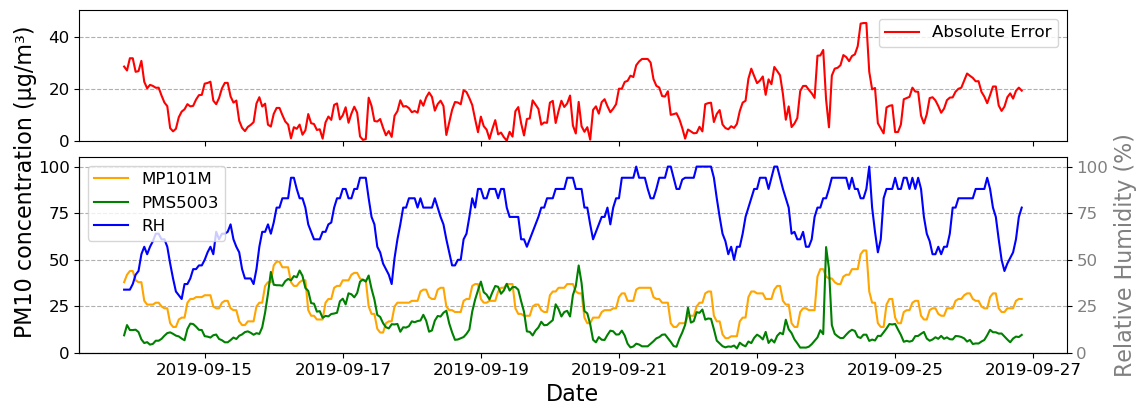
\includegraphics[width=0.9\textwidth]{./Images/calibration-thin-article.png}
\caption{PM10 concentrations reported by the sensors and RH.}
\label{fig:system-calibration}
\end{figure*}

The scatter diagram in Figure \ref{fig:scatter-measurements} shows that the developed system measured values are predominantly lower than the reference readings.

\setlength{\abovecaptionskip}{10pt plus 0pt minus 0pt}
\begin{figure}[ht]
\centering
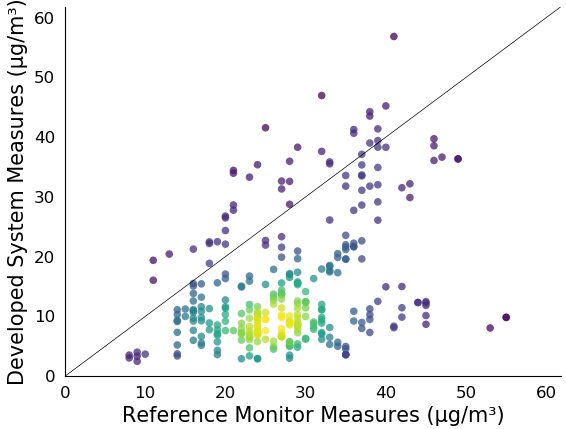
\includegraphics[width=0.45\textwidth]{./Images/scatter-measurements.png}
\caption{Scatter diagram between the developed system and the reference monitor measures.}
\label{fig:scatter-measurements}
\end{figure}

In the comparison of time series data, it is important to assess not only the error statistics between datasets, but also its linearity and correlation. 

The Pearson coefficient was calculated for every full day of the time series data, during the developed sensor placement. The coefficient obtained for the whole period was 0.39, with several days presenting negative correlation coefficients between measures.

%\begin{table*}[ht]
%\footnotesize
%\centering
%\caption{Pearson coefficients calculated for the %full days of sensor positioning.}
%\label{table:pearson-coefs-sensor}
%\begin{tabular}[t]{>{\centering}p{0.06\linewidth%}>{\centering}p{0.06\linewidth}>{\centering\arra%ybackslash}>{\centering}p{0.06\linewidth}>{\cent%ering}p{0.06\linewidth}>{\centering}p{0.06\linew%idth}>{\centering}p{0.06\linewidth}>{\centering}%p{0.06\linewidth}>{\centering}p{0.06\linewidth}>%{\centering}p{0.06\linewidth}>{\centering}p{0.06%\linewidth}>{\centering}p{0.06\linewidth}>{\cent%ering}>{\centering}p{0.06\linewidth}>{\centering%\arraybackslash}p{0.1\linewidth}}
%\toprule
%\multicolumn{12}{c}{Day of %placement}&\multirow{2}{*}{Overall}\\\cline{1-12%}
%1&2&3&4&5&6&7&8&9&10&11&12&\\
%\midrule
%0.22&0.57&0.68&0.60&0.75&0.62&0.59&-0.23&0.57  %&0.34&0.01&-0.37&0.39\\
%\bottomrule
%\end{tabular}
%\end{table*}%

\subsection{SIMs Testing}

In this section, every SIM performance test result is presented.

Through the cross validation approach application in the dataset, the IDW power function was tested with values between 0 and 5, and the value with the best error statistics was \textit{p} = 0. 

The same approach was applied in the parameter assessment of the remaining algorithms. In OK, the variogram is the main user-defined parameter. Several pre-defined variograms were tested, and in the obtained results the linear model had the lowest overall MAE and RMSE values.

In what regards FBN interpolation, both testing and training epochs, network size, number of samples and granularity of the memories of each consequent neuron were tested. The chosen parameters were 30, 30, 75, 9 and 3, respectively.

\subsubsection{SIMs Comparison}

Results regarding MAE and RMSE performance are presented in table Table \ref{table:sim-comparison}, for each algorithm and each target station, for a total of 43 956 inferences.

\begin{table}[H]
\centering
\footnotesize
\caption{Model comparison results.}
\label{table:sim-comparison}
\begin{tabular}[t]{l>{\centering}p{0.075\linewidth}>{\centering}p{0.088\linewidth}>{\centering}p{0.08\linewidth}>{\centering}p{0.088\linewidth}>{\centering}p{0.08\linewidth}>{\centering}p{0.088\linewidth}>{\centering}p{0.08\linewidth}>{\centering\arraybackslash}p{0.088\linewidth}}
\toprule
&\multicolumn{2}{c}{ENC}&\multicolumn{2}{c}{ODI}&\multicolumn{2}{c}{REB}&\multicolumn{2}{c}{SCB}\\
\midrule
{} &MAE&RMSE&MAE&RMSE&MAE&RMSE&MAE&RMSE\\
\midrule
IDW&4.65&6.52&4.89&6.48&5.46&6.97&11.52&15.31\\
OK&4.67&6.52&4.89&6.49&5.55&7.06&11.41&15.18\\
FBN&5.82&7.62&6.36&8.41&7.55&9.62&11.08&14.75\\
Linear&5.90&7.74&6.59&9.46&10.11&13.11&11.04&14.51\\
NearestN&11.20&14.63&7.35&9.82&12.58&16.36&13.45&17.22\\
\bottomrule
\end{tabular}
\end{table}

The algorithms with overall lower MAE and RMSE results were IDW and OK. NN had the worse results, followed by LI. Histograms resulting from the IDW, OK and FBN execution can be observed in Figure \ref{fig:performance-histograms}.

\begin{figure}[ht]
\centering
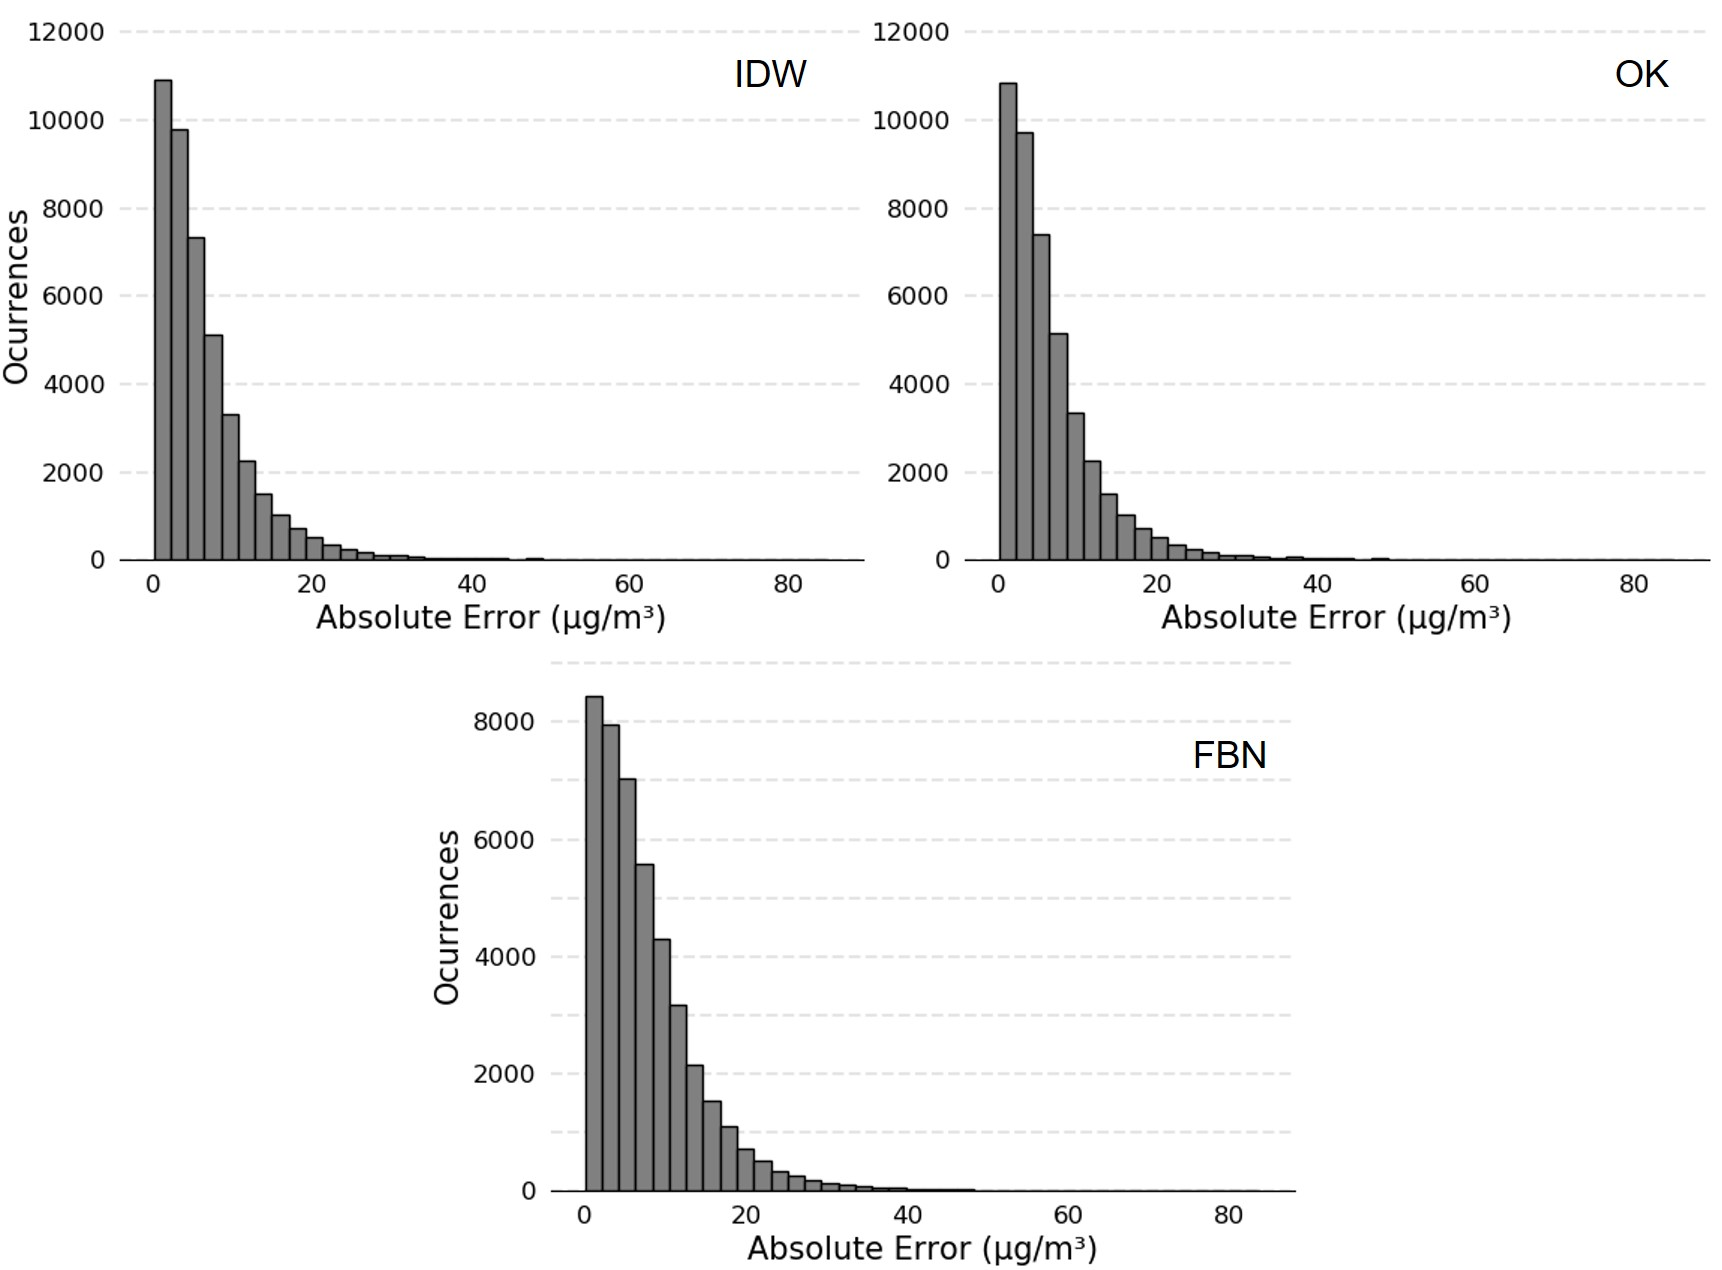
\includegraphics[width=0.49\textwidth]{./Images/performance-histograms.jpg}
\caption{Histograms obtained from 43 956 inferences for IDW, OK and FBN.}
\label{fig:performance-histograms}
\end{figure}

It should additionally be noted that, for all the inferences done simultaneously, FBNs execution times were around 9 hours, while remaining algorithms only took from approximately 5 minutes.

\subsection{Online Data Visualization Web Application}

The resulting PM10 visualization application has a resolution of 100 meters, both in color and in height of the pollution surface. It provides the possibility to hover over the grid to consult estimated PM10 concentration values in any location inside the outline defined by the CCDR-LVT monitoring network stations.

The application design is focused in the user experience, and allows the user to zoom in and out, and change both pitch and bearing of the map. The final result of the developed web application is presented in Figure \ref{fig:developed-visualization}.

\begin{figure}[ht]
\centering
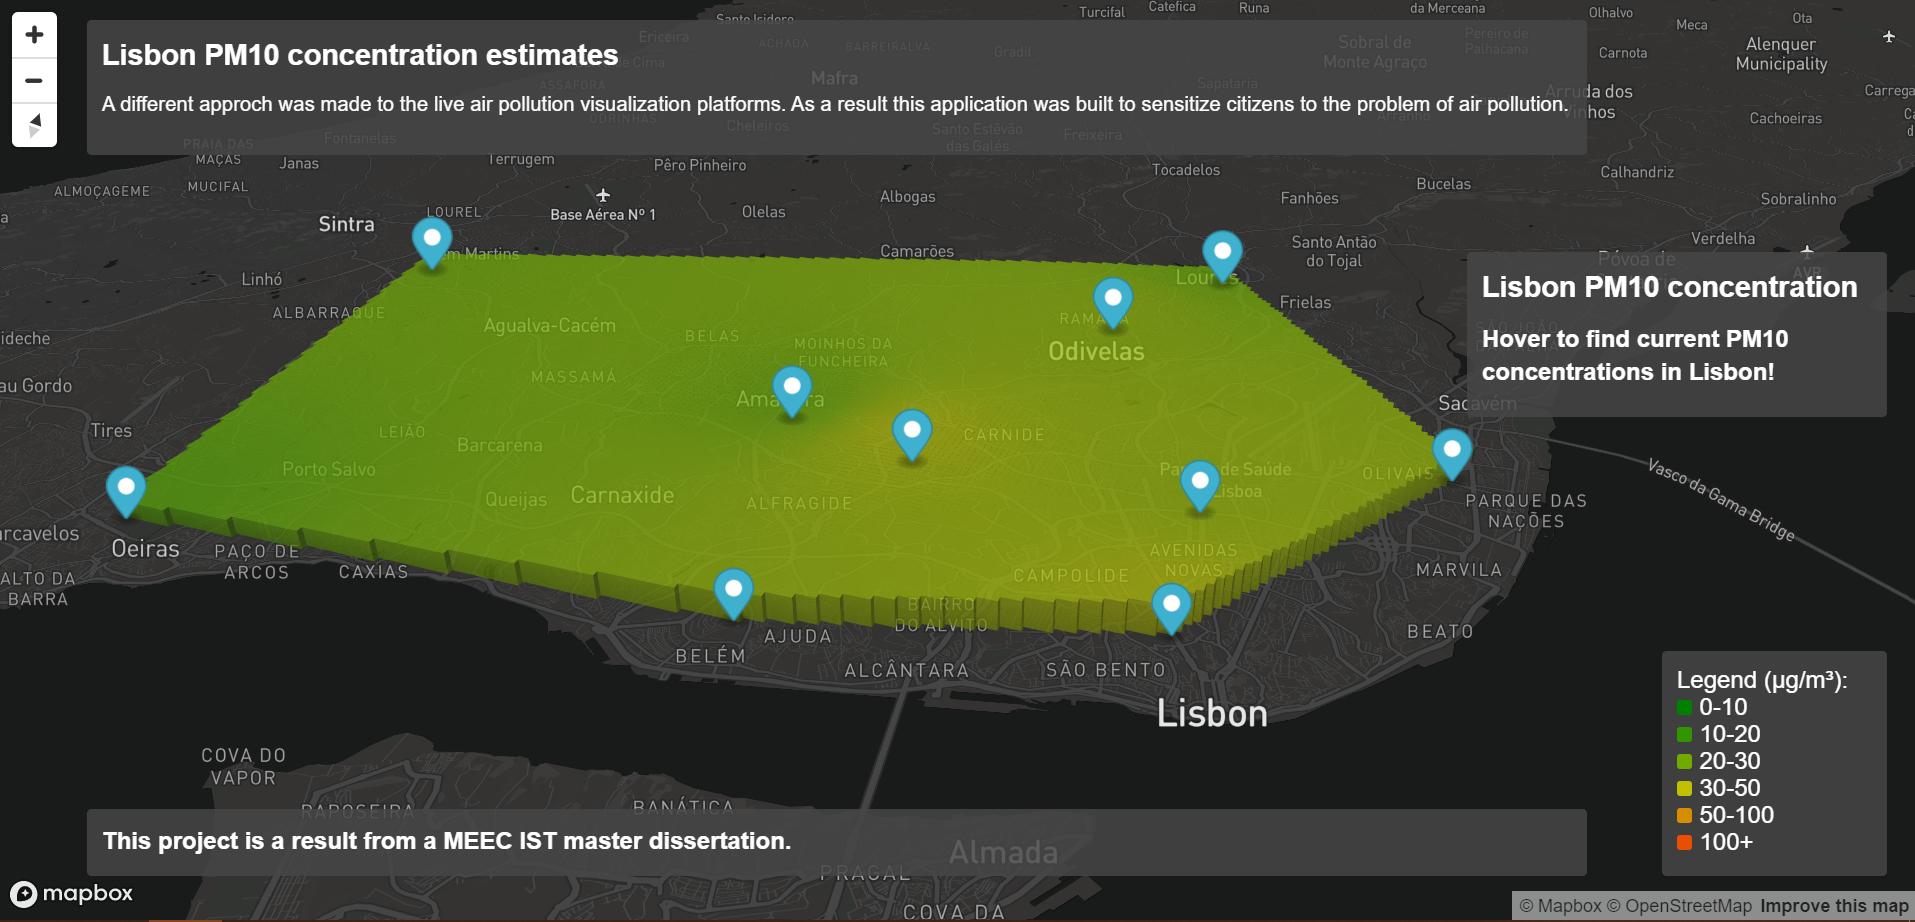
\includegraphics[width=0.49\textwidth]{./Images/developed-visualization.PNG}
\caption{Developed Web Application final result.}
\label{fig:developed-visualization}
\end{figure}

\subsection{Discussion}

%Results obtained and presented in this chapter are discussed in this section regarding every stage of this work.

\subsubsection{Developed PM10 Monitoring System}

Regarding the NB-IoT coverage in Portugal, from both MEO and NOS, namely in the capital Lisbon, it was observed that it was not good enough for professional applications at the time of this work. During the 10 weeks of testing in different locations in the city of Lisbon, there were only 2 weeks when it was possible to get consistent coverage. According to the literature \cite{Lauridsen2017}, NB-IoT has one of the widest coverage between IoT technologies. This was not observed in this work. Results demonstrated that the developed sensor, at the time of this work, from the network coverage perspective, can not be employed neither integrate current official monitoring networks.

Before assessing measurement performance, it is important to note that the obtained data only corresponds to a small sample size in comparison to what was expected.

% observations + error statistics

As mentioned, during the sensor placement and comparison period, the PMS5003 sensor often obtained lower measures (Figure \ref{fig:scatter-measurements}). However, sometimes it peaked, surpassing the MP101M measures. This only happened for high values of RH. It could additionally be observed, in Figure \ref{fig:system-calibration}, that when the RH is decreasing, there is often less error is observed between the sensors.

The average absolute error between the measures of the different sensors (14.40 $\mu g/m^3$) is slightly above the smallest scale division of the classification in Table \ref{table:pm10-classification}. The daily pearson correlation coefficients showed inconsistency in the linearity between sensor readings.

It was summer season during this experiment, and the only rain occurrences during the placement periods happened in the day 21 of September. It was the day with the second highest absolute error between readings and PMS5003 measured values were lower than average in comparison to the reference sensor.

% humidity
In a study by Zheng et al., in 2018, a similar sensor model (PMS3003) was extensively tested and it was observed that while temperature took a negligible part in the difference observed between sensors, RH had a much more considerable influence \cite{Zheng2018}. 

The registered high humidity intervals correspond to night and dawn periods. 
Similar to what happened in a study by Jayaratne et al., in 2018, in these periods, measures are often higher than in the rest of the time.

In the same study, it was stated that above 75\% RH, marked effects are seen in low-cost sensors due to air particle size growth by deliquescence, specially if these do not have drying facilities at the sample inlets \cite{Jayaratne2018}. However, in this work, the only observed effects were the readings increase, which was also reported by the MP101M, and the mentioned undervalued PMS5003 measurements during the rain periods.

% car traffic
No substantial difference was observed between week and weekend days, despite the average PM10 concentration being slightly lower in both sensors.

During the day, MP101M readings are mostly higher than the taken by PMS5003.
According to Jayaratne et al., in the same study \cite{Jayaratne2018}, this may happen because the size of traffic particles are below the minimum detectable size limit of the PMS sensors. It is documented that the diameter of particles emitted by vehicles can be mostly below 300 nm \cite{Li2018}.

% conclusion on placement in official networks
Due to the numerous disadvantages observed with data from this work, it can be inferred that low-cost sensors are not suited for regulatory applications, such as assessing if the air quality meets stipulated guidelines. However, with previous study of the placement location and the deduction of a fitting correction factor to each case, it could be implemented for informative purposes, such as providing a better resolution to monitoring networks which suffer from sparsity.

%%%%

\subsubsection{SIMs Assessment}

The algorithms with the best performance overall were IDW and OK, followed by FBNs, LI and lastly NN.

In Table \ref{table:correlation-coef}, correlation coefficients between every station of the dataset were calculated. It can be observed that the stations with shared highest correlation coefficients were relatively close in terms of geographical location, despite an overall high correlation between almost every station. However, the good performance of IDW with \textit{p} = 0, which means that distance between data points is not considered for the interpolation, suggests that the spatial correlation between stations is very low.

Air dispersion and movement in urban environments is an environmental problem of high complexity. In the last 5 years, in the city of Lisbon, the dataset reveals that the city of Lisbon has an overall low concentration of PM10, with a maximum mean value for the whole dataset of 34.22 $\mu g/m^3$ in the station of Avenida da Liberdade, which is a value classified as \textit{Good}.

The fact that these SIMs were tested for periods where no big pollution phenomena affected the city, could degrade the sense of spatial correlation between the stations in the city, because the collected data was predominantly constant and similar between stations, as is the IDW interpolation.

Several other environmental factors can have influenced the spatial correlation of PM10 concentration throughout the city, such as the wind direction, the temperature, humidity, the altitude of the interpolation point and the traffic density and pollution, as well as the presence of buildings and other geological and geographical barriers to airflow.

In what regards FBNs performance, no conclusions can be obtained towards its performance regarding multidimensional spatial interpolation problems, due to the low spatial correlation between the data points of the performed experiments. However, it can be concluded that FBNs are not suitable for problems which require real time interpolations with fast computations and construction of interpolation surfaces, due to the observed high computing times.

\subsubsection{Web Visualization Application}

The developed application resulted in a platform with the presentation of live PM10 concentration data with high resolution in the area covered by the CCDR-LVT monitoring stations network in Lisbon. Since results obtained from the low-cost sensors reveal these are not yet suitable to be integrated on monitoring networks, these were not included in the network used for the spatial interpolation presented in the application.

The application is flexible from a development point of view. It can easily be extended to support several other air polluting gases concentration or indicators. The same structure could be applied in other geographical interpolation fields.

In comparison with current governmental web applications available, the developed application has higher resolution and provides better user experience, despite not covering large areas such as whole countries. As a product, there are already companies with applications which outperform it, being the most evident Breezometer. It presents data regarding numerous air polluting gases and indicators with a resolution of 500 meters, and worldwide coverage. However, due to its proprietary characteristics, its air modelling algorithms and tools are not documented and consequently not available for assessment.


%%%%%%%%%%%%%%%%%%%%%%%%%%%%%%%%%%%%%%%%%%%%%%%%%%%%%%%%%%%%%%%%%%%%%%
% CONCLUSIONS
%%%%%%%%%%%%%%%%%%%%%%%%%%%%%%%%%%%%%%%%%%%%%%%%%%%%%%%%%%%%%%%%%%%%%%
\section{Conclusions}
\label{sec:concl}

The current state of the data available publicly regarding air quality was studied and assessed. Several experiments were made in order to evaluate the application of new technologies which could improve it. The tested PMS5003 low-cost PM sensor did not show promising results for official networks integration, and requires complex calibration in order to be used for interpolation purposes. 

Spatial interpolation algorithms showed a low spatial correlation, due to the sparsity of the stations in the city, adding to the importance of the study of lower-cost sensors integration. 

It can be concluded that the developed visualization platform could bring awareness to the citizens in what regards their cities air quality, in high resolution, and constitute a replacement for current government platforms.

Relevant results were obtained regarding the usage and performance of every technology used and applied in this work. Finally, information was gathered for further study of the phenomenon of spatial interpolation of air quality, its measurement and its visualization.

\subsection{Future Work}

In a study using NB-IoT, several tests and an evaluation of the study area coverage should be made previously to its application. Low-cost PM monitoring sensors should be further studied in controlled environments. Ideally, with a  calibration function which could minimize the error to extremely low values, for each specific placement location, this type of sensors could integrate air quality monitoring network for interpolation purposes.

Spatial algorithms tested in this work could be complemented with the addition of other independent variables, besides coordinates, and air dispersion models. FBN implementation could be parallelized, and further studied regarding spatial geographical interpolation with the integration of additional variables to the problem.

%%%%%%%%%%%%%%%%%%%%%%%%%%%%%%%%%%%%%%%%%%%%%%%%%%%%%%%%%%%%%%%%%%%%%%
% ACKNOWLEDGMENTS
%%%%%%%%%%%%%%%%%%%%%%%%%%%%%%%%%%%%%%%%%%%%%%%%%%%%%%%%%%%%%%%%%%%%%%
%%%%%%%%%%%%%%%%%%%%%%%%%%%%%%%%%%%%%%%%%%%%%%%%%%%%%%%%%%%%%%%%%%%%%%
%     File: ExtendedAbstract_ackno.tex                               %
%     Tex Master: ExtendedAbstract.tex                               %
%                                                                    %
%     Author: Andre Calado Marta                                     %
%     Last modified : 27 Dez 2011                                    %
%%%%%%%%%%%%%%%%%%%%%%%%%%%%%%%%%%%%%%%%%%%%%%%%%%%%%%%%%%%%%%%%%%%%%%
% Acknowledge persons and institutions that supported this work.
%%%%%%%%%%%%%%%%%%%%%%%%%%%%%%%%%%%%%%%%%%%%%%%%%%%%%%%%%%%%%%%%%%%%%%

%\section*{Acknowledgements}

%The author would like to thank ...



%%%%%%%%%%%%%%%%%%%%%%%%%%%%%%%%%%%%%%%%%%%%%%%%%%%%%%%%%%%%%%%%%%%%%%
% REFERENCES
%%%%%%%%%%%%%%%%%%%%%%%%%%%%%%%%%%%%%%%%%%%%%%%%%%%%%%%%%%%%%%%%%%%%%%

% Produces the bibliography section when processed by BibTeX
%
% Bibliography style
% > entries ordered alphabetically
%\bibliographystyle{plain}
% > unsorted with entries appearing in the order in which the citations appear.
%\bibliographystyle{unsrt}
% > entries ordered alphabetically, with first names and names of journals and months abbreviated
\bibliographystyle{abbrv}
% > entries ordered alphabetically, with reference markers based on authors' initials and publication year
%\bibliographystyle{alpha}

% External bibliography database file in the BibTeX format (ExtendedAbstract_ref_db.bib)
\bibliography{ExtendedAbstract_ref_db}

%%%%%%%%%%%%%%%%%%%%%%%%%%%%%%%%%%%%%%%%%%%%%%%%%%%%%%%%%%%%%%%%%%%%%%
\end{document}
%%%%%%%%%%%%%%%%%%%%%%%%%%%%%%%%%%%%%%%%%%%%%%%%%%%%%%%%%%%%%%%%%%%%%%

